\begin{exercise}{8}
	Let $X, Y$ and $Z$ be global variables in the program given below.
	
   \begin{lstlisting}[language=Java, caption=A simple pointer program.]
   class Node {
      Node* left = NULL;
      int value = 0;
      Node* right = NULL;

      public Node(int v) { this.value = v; }
   }
   
   Node* X := NULL;
   Node* Y := NULL;
   Node* Z := NULL;
   
   func main() {
      X := new Node(1);
      X.left = X;
      X.right = new Node(2);
      Y := X.right;
      Z := getTree(Y); // see heap diagram for result
	
      // <-- The heap presented belongs to the program in this state

      X := new Node(3);
      X.left := new Node(4);
      X.value = 42;
      X.right := new Node(5);
      Z.left := NULL;
   }
   \end{lstlisting}
  
  \begin{figure}[h]
  	\centering
  	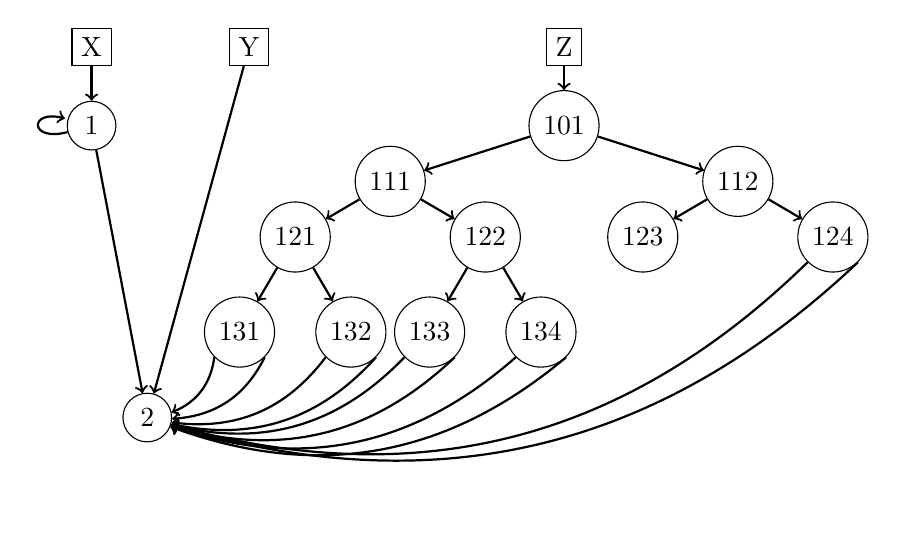
\begin{tikzpicture}
  	\node[draw,] at (0,0) (rootX) {X};
  	\node[draw,circle,below of=rootX] (XN) {1};
  	\node[draw,circle,below right of=XN,yshift=-3.0cm] (XrN) {2};
  	
  	\node[draw,] at (2,0) (rootY) {Y};
  	
  	\node[draw,xshift=2.0cm] at (4,0) (rootZ) {Z};
  	\node[draw,circle,below of=rootZ] (Z-0-N) {101};
  	\node[draw,circle,below left of=Z-0-N,xshift=-1.5cm] (Z-1-N1) {111};
  	\node[draw,circle,below right of=Z-0-N,xshift=1.5cm] (Z-1-N2) {112};
  	
  	\node[draw,circle,below left of=Z-1-N1,xshift=-0.5cm] (Z-2-N1) {121};
  	\node[draw,circle,below right of=Z-1-N1,xshift=0.5cm] (Z-2-N2) {122};
  	
  	\node[draw,circle,below left of=Z-1-N2,xshift=-0.5cm] (Z-2-N3) {123};
  	\node[draw,circle,below right of=Z-1-N2,xshift=0.5cm] (Z-2-N4) {124};
  	
  	\node[draw,circle,below left of=Z-2-N1,yshift=-0.5cm] (Z-3-N1) {131};
  	\node[draw,circle,below right of=Z-2-N1,yshift=-0.5cm] (Z-3-N2) {132};
  	
  	\node[draw,circle,below left of=Z-2-N2,yshift=-0.5cm] (Z-3-N3) {133};
  	\node[draw,circle,below right of=Z-2-N2,yshift=-0.5cm] (Z-3-N4) {134};
  	
  	\path[]
  	   (rootX) edge [->,thick] (XN)
  	   (XN) edge [loop left, thick] (XN)
  	   (XN) edge[->,thick] (XrN)
  	   
  	   (rootY) edge[->,thick] (XrN)
  	   
  	   (rootZ) edge [->,thick] (Z-0-N)
  	   (Z-0-N) edge [->,thick] (Z-1-N1)
  	   (Z-0-N) edge [->,thick] (Z-1-N2)
  	   
  	   (Z-1-N1) edge [->,thick] (Z-2-N1)
  	   (Z-1-N1) edge [->,thick] (Z-2-N2)
  	   
  	   (Z-1-N2) edge [->,thick] (Z-2-N3)
  	   (Z-1-N2) edge [->,thick] (Z-2-N4)
  	   
  	   (Z-2-N1) edge [->,thick] (Z-3-N1)
  	   (Z-2-N1) edge [->,thick] (Z-3-N2)
  	   
  	   (Z-2-N2) edge [->,thick] (Z-3-N3)
  	   (Z-2-N2) edge [->,thick] (Z-3-N4)
  	   
  	   
  	   (Z-3-N1.-45) edge [->,thick, bend left] (XrN)
  	   (Z-3-N2.-45) edge [->,thick, bend left] (XrN)  	   
  	   (Z-3-N3.-45) edge [->,thick, bend left] (XrN)
  	   (Z-3-N4.-45) edge [->,thick, bend left] (XrN)
  	   (Z-3-N1.-135) edge [->,thick, bend left] (XrN)
  	   (Z-3-N2.-135) edge [->,thick, bend left] (XrN)  	   
  	   (Z-3-N3.-135) edge [->,thick, bend left] (XrN)
  	   (Z-3-N4.-135) edge [->,thick, bend left] (XrN)
  	   
  	   (Z-2-N4.-45) edge [->,thick, bend left] (XrN)
   	   (Z-2-N4.-135) edge [->,thick, bend left] (XrN)
  	   ;
  	\end{tikzpicture}
  	%(Z-2-N3.-45) edge [->,thick, bend left] (XrN)
  	%(Z-2-N3.-135) edge [->,thick, bend left] (XrN)
  	
  	
  	\caption{The state of the heap at the marked program location.}
  \end{figure}

  \begin{enumerate}
    \item[(a)] Calculate the reference count for each object \texttt{Node} at the marked location in the program. 
    \item[(b)] Show the heap after executing the remaining statements of \texttt{main()}, including the reference counts, but before any garbage collection has occurred.
    \item[(c)] Perform a garbage collection run using mark-and-sweep and indicate which nodes get ``collected'' by drawing the resulting heap.
    \item[(d)] Perform a garbage collection run using reference counting and indicate which nodes get ``collected'' by drawing the resulting heap.
  \end{enumerate}
\end{exercise}

\begin{solution}
  \begin{enumerate}
    \item[(a)]
    	\begin{tabular}[t]{|l c|}
    		\hline
    		Node & Ref. Count\\
    		\hline
    		1 & 2\\
    		2 & 12\\
    		101 ... 134 & 1\\
    		\hline
    	\end{tabular}
    
    \item[(b)] See Figure \ref{fig:solutionB} for the heap structure.\\
    \begin{tabular}{|l c| }
    	\hline
    	Node & Ref. Count\\
    	\hline
    	1 & 1\\
    	2 & 12\\
    	4 & 1\\
    	5 & 1\\
    	42 & 1\\
    	101 & 1\\
    	111 & 0\\
    	112 ... 134 & 1\\
    	\hline
    \end{tabular}
    
    \begin{figure}[h]
    	\centering
    	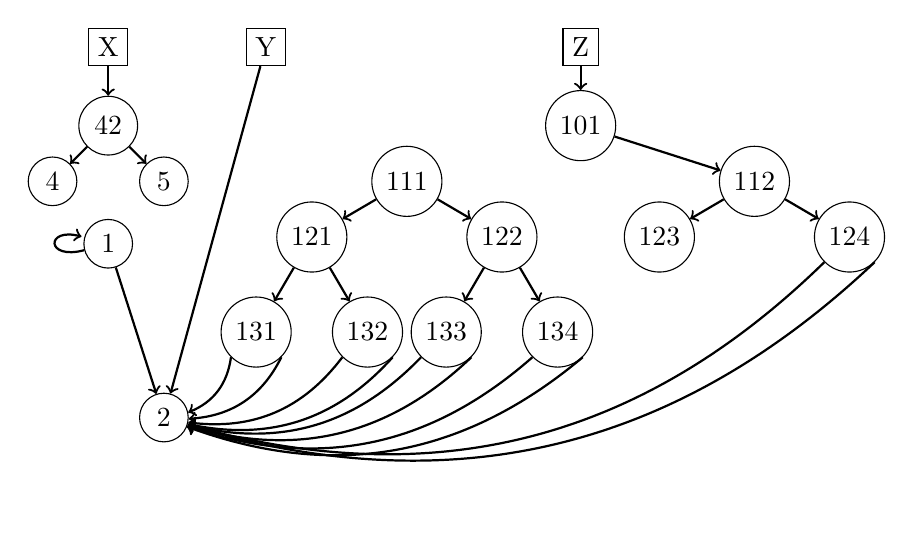
\begin{tikzpicture}
    	\node[draw,] at (0,0) (rootX) {X};
    	\node[draw,circle,below of=rootX] (XN) {42};
    	\node[draw,circle,below left of=XN] (XlC) {4};
    	\node[draw,circle,below right of=XN] (XrC) {5};
    	
    	\node[draw,circle,below of=rootX,yshift=-1.5cm] (XNold) {1};
    	\node[draw,circle,below right of=XN,yshift=-3.0cm] (XrN) {2};
    	
    	\node[draw,] at (2,0) (rootY) {Y};
    	
    	\node[draw,xshift=2.0cm] at (4,0) (rootZ) {Z};
    	\node[draw,circle,below of=rootZ] (Z-0-N) {101};
    	\node[draw,circle,below left of=Z-0-N,xshift=-1.5cm] (Z-1-N1) {111};
    	\node[draw,circle,below right of=Z-0-N,xshift=1.5cm] (Z-1-N2) {112};
    	
    	\node[draw,circle,below left of=Z-1-N1,xshift=-0.5cm] (Z-2-N1) {121};
    	\node[draw,circle,below right of=Z-1-N1,xshift=0.5cm] (Z-2-N2) {122};
    	
    	\node[draw,circle,below left of=Z-1-N2,xshift=-0.5cm] (Z-2-N3) {123};
    	\node[draw,circle,below right of=Z-1-N2,xshift=0.5cm] (Z-2-N4) {124};
    	
    	\node[draw,circle,below left of=Z-2-N1,yshift=-0.5cm] (Z-3-N1) {131};
    	\node[draw,circle,below right of=Z-2-N1,yshift=-0.5cm] (Z-3-N2) {132};
    	
    	\node[draw,circle,below left of=Z-2-N2,yshift=-0.5cm] (Z-3-N3) {133};
    	\node[draw,circle,below right of=Z-2-N2,yshift=-0.5cm] (Z-3-N4) {134};
    	
    	\path[]
    	(rootX) edge [->,thick] (XN)
    	(XN) edge[->,thick] (XlC)
    	(XN) edge[->,thick] (XrC)
    	
    	(XNold) edge [loop left, thick] (XNold)
    	(XNold) edge[->,thick] (XrN)
    	
    	(rootY) edge[->,thick] (XrN)
    	
    	(rootZ) edge [->,thick] (Z-0-N)
    	(Z-0-N) edge [->,thick] (Z-1-N2)
    	
    	(Z-1-N1) edge [->,thick] (Z-2-N1)
    	(Z-1-N1) edge [->,thick] (Z-2-N2)
    	
    	(Z-1-N2) edge [->,thick] (Z-2-N3)
    	(Z-1-N2) edge [->,thick] (Z-2-N4)
    	
    	(Z-2-N1) edge [->,thick] (Z-3-N1)
    	(Z-2-N1) edge [->,thick] (Z-3-N2)
    	
    	(Z-2-N2) edge [->,thick] (Z-3-N3)
    	(Z-2-N2) edge [->,thick] (Z-3-N4)
    	
    	
    	(Z-3-N1.-45) edge [->,thick, bend left] (XrN)
    	(Z-3-N2.-45) edge [->,thick, bend left] (XrN)  	   
    	(Z-3-N3.-45) edge [->,thick, bend left] (XrN)
    	(Z-3-N4.-45) edge [->,thick, bend left] (XrN)
    	(Z-3-N1.-135) edge [->,thick, bend left] (XrN)
    	(Z-3-N2.-135) edge [->,thick, bend left] (XrN)  	   
    	(Z-3-N3.-135) edge [->,thick, bend left] (XrN)
    	(Z-3-N4.-135) edge [->,thick, bend left] (XrN)
    	
    	(Z-2-N4.-45) edge [->,thick, bend left] (XrN)
    	(Z-2-N4.-135) edge [->,thick, bend left] (XrN)
    	;
    	\end{tikzpicture}
    	%(Z-2-N3.-45) edge [->,thick, bend left] (XrN)
    	%(Z-2-N3.-135) edge [->,thick, bend left] (XrN)
    	
    	
    	\caption{The state of the heap at the end of \texttt{main}.}
    	\label{fig:solutionB}
    \end{figure}
    
    \item[(c)] 
    \begin{enumerate}
    	\item Marking phase.
    	\begin{itemize}
    		\item Object X: Reachable nodes are $42, 4$ and $5$.
   			\item Object Y: The only reachable node is $2$.
   			\item Object Z: Reachable nodes are $101, 112, 123, 124$ and $2$.
    	\end{itemize}
    	The merged set of all reachable nodes is $\{ 2, 4, 5, 42, 101, 112, 123, 124 \}$.
    	\item Sweep phase.\\
    	Collected objects are $\{ 1, 111, 121, 122, 131, 132, 133, 134 \}$.
    	See Figure \ref{fig:solutionC} for the resulting heap.
    	
    	\begin{figure}[h]
    		\centering
    		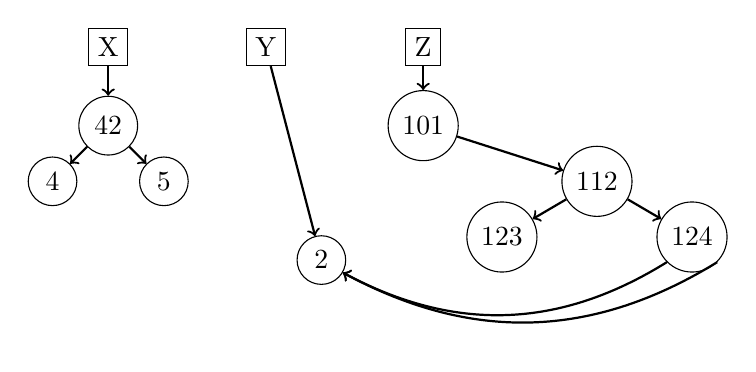
\begin{tikzpicture}
    		\node[draw,] at (0,0) (rootX) {X};
    		\node[draw,circle,below of=rootX] (XN) {42};
    		\node[draw,circle,below left of=XN] (XlC) {4};
    		\node[draw,circle,below right of=XN] (XrC) {5};
    		
    		
    		\node[draw,] at (2,0) (rootY) {Y};
    		\node[draw,circle,below right of=rootY,yshift=-2.0cm] (XrN) {2};
    		
    		\node[draw,xshift=0.0cm] at (4,0) (rootZ) {Z};
    		\node[draw,circle,below of=rootZ] (Z-0-N) {101};
    		\node[draw,circle,below right of=Z-0-N,xshift=1.5cm] (Z-1-N2) {112};
    		    		
    		\node[draw,circle,below left of=Z-1-N2,xshift=-0.5cm] (Z-2-N3) {123};
    		\node[draw,circle,below right of=Z-1-N2,xshift=0.5cm] (Z-2-N4) {124};
    		
    		\path[]
    		(rootX) edge [->,thick] (XN)
    		(XN) edge[->,thick] (XlC)
    		(XN) edge[->,thick] (XrC)
    		    		
    		(rootY) edge[->,thick] (XrN)
    		
    		(rootZ) edge [->,thick] (Z-0-N)
    		(Z-0-N) edge [->,thick] (Z-1-N2)
    		    		
    		(Z-1-N2) edge [->,thick] (Z-2-N3)
    		(Z-1-N2) edge [->,thick] (Z-2-N4)
		
    		(Z-2-N4.-45) edge [->,thick, bend left] (XrN)
    		(Z-2-N4.-135) edge [->,thick, bend left] (XrN)
    		;
    		\end{tikzpicture}
    		%(Z-2-N3.-45) edge [->,thick, bend left] (XrN)
    		%(Z-2-N3.-135) edge [->,thick, bend left] (XrN)
    		
    		
    		\caption{The state of the heap after garbage collection using mark-and-sweep.}
    		\label{fig:solutionC}
    	\end{figure}
    \end{enumerate}
    \item[(d)] Using the reference counts obtained in (b), we can see that only node $111$ is immediately eligible for garbage collection. After deleting the node and adjusting reference counts accordingly, the nodes $121$ and $122$ become eligible, followed by their successors $131, 132, 133$ and $134$. This brings the reference count of $2$ down to $4$, and collection terminates. See Figure \ref{fig:solutionD} for the resulting heap.
    
    \begin{figure}[h]
    	\centering
    	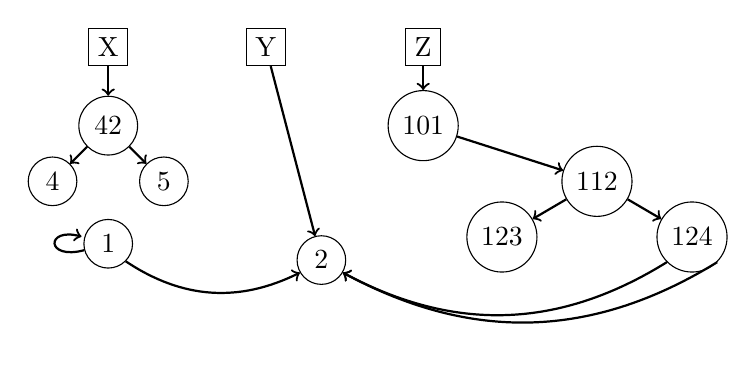
\begin{tikzpicture}
    	\node[draw,] at (0,0) (rootX) {X};
    	\node[draw,circle,below of=rootX] (XN) {42};
    	\node[draw,circle,below left of=XN] (XlC) {4};
    	\node[draw,circle,below right of=XN] (XrC) {5};
    	
    	\node[draw,circle,below of=rootX,yshift=-1.5cm] (XNold) {1};
    	
    	\node[draw,] at (2,0) (rootY) {Y};
    	\node[draw,circle,below right of=rootY,yshift=-2.0cm] (XrN) {2};
    	
    	\node[draw,xshift=0.0cm] at (4,0) (rootZ) {Z};
    	\node[draw,circle,below of=rootZ] (Z-0-N) {101};
    	\node[draw,circle,below right of=Z-0-N,xshift=1.5cm] (Z-1-N2) {112};
    	    	
    	\node[draw,circle,below left of=Z-1-N2,xshift=-0.5cm] (Z-2-N3) {123};
    	\node[draw,circle,below right of=Z-1-N2,xshift=0.5cm] (Z-2-N4) {124};
    	
    	\path[]
    	(rootX) edge [->,thick] (XN)
    	(XN) edge[->,thick] (XlC)
    	(XN) edge[->,thick] (XrC)
    	
    	(XNold) edge [loop left, thick] (XNold)
    	(XNold.-45) edge[->,thick, bend right] (XrN)
    	
    	(rootY) edge[->,thick] (XrN)
    	
    	(rootZ) edge [->,thick] (Z-0-N)
    	(Z-0-N) edge [->,thick] (Z-1-N2)
    	
    	(Z-1-N2) edge [->,thick] (Z-2-N3)
    	(Z-1-N2) edge [->,thick] (Z-2-N4)

    	(Z-2-N4.-45) edge [->,thick, bend left] (XrN)
    	(Z-2-N4.-135) edge [->,thick, bend left] (XrN)
    	;
    	\end{tikzpicture}
    	%(Z-2-N3.-45) edge [->,thick, bend left] (XrN)
    	%(Z-2-N3.-135) edge [->,thick, bend left] (XrN)
    	
    	
    	\caption{The state of the heap after garbage collection using reference counting.}
    	\label{fig:solutionD}
    \end{figure}
  \end{enumerate}
\end{solution}
